\documentclass{beamer}
\usepackage[utf8]{inputenc}
\usepackage{amsmath, mathrsfs, mathtext, bm}
\usepackage{graphicx, epsfig, float}
\usepackage{fancybox}
\usepackage{amsfonts}
\usepackage{fancyhdr}
\usepackage{array}
\usepackage{makecell}
\usepackage{colortbl}
\usepackage{hhline}
\usepackage{subfig}
\usepackage{epstopdf}
\usepackage{tikz}
\usepackage{pgfplots}

\usepackage{algorithm, algorithmic}
\renewcommand{\algorithmicrequire}{\textbf{Input:}}
\renewcommand{\algorithmicensure}{\textbf{Output:}}

\newcommand\blfootnote[1]{%
	\begingroup
	\renewcommand\thefootnote{}\footnote{#1}%
	\addtocounter{footnote}{-1}%
	\endgroup
}

\setbeamerfont{footnote}{size=\tiny}

\newcommand\abs[1]{\left|#1\right|}
\newcommand{\x}{\mathbf{x}}
\newcommand{\MyMatrix}[1]{\bm{\mathit{#1}}}
\DeclareMathOperator{\sgn}{\mathop{sgn}}
\DeclareMathOperator*{\argmin}{arg\,min}
\DeclareMathOperator*{\argmax}{arg\,max}

\usetheme{Boadilla}%{Singapore}%{Warsaw}%{Warsaw}%{Darmstadt}
\usecolortheme{default}
\useoutertheme{split}
% ��������� ������� ���������
\setbeamertemplate{navigation symbols}{}


\title[Structure learning\hspace{25mm} \insertframenumber/\inserttotalframenumber]{Structure learning for model generation}
\author[Bochkarev A.]{Artem Bochkarev\\
Advisors: Maxim Fedorov, Vadim Strijov}
\date{}
\institute[Skoltech, MIPT]{Skolkovo Institute of Science and Technology\\
	Moscow Institute of Physics and Technology
    \vspace{0.3cm}
}

\date{}

\begin{document}


% Creates title page of slide show using above information
\begin{frame}
  \titlepage
\end{frame}


\begin{frame}{Introduction}
\begin{block}{Problem}
	\begin{itemize}
		\item Building machine learning models is not automated
		\item Symbolic regression is a computationally heavy algorithm
	\end{itemize}
\end{block}

\begin{block}{Aim and objectives}
	\begin{itemize}
		\item Automate building symbolic regression models
		\item Explore meta learning approach for symbolic regression
	\end{itemize}
\end{block}
\end{frame}

\begin{frame}{Literature}
\begin{itemize}
	\item Genetic programming \begin{itemize}
		\item Kulunchakov, A. S., \& Strijov, V. V. (2017). Generation of simple structured information retrieval functions by genetic algorithm without stagnation. \textit{Expert Systems with Applications, 85, 221-230.}
		\item Koza, J. R. (1994). Genetic programming as a means for programming computers by natural selection. \textit{Statistics and computing, 4(2), 87-112.}
	\end{itemize}

	\item Meta learning \begin{itemize}
		\item Zoph, B., \& Le, Q. V. (2016). Neural architecture search with reinforcement learning. \textit{arXiv preprint arXiv:1611.01578.}
		\item Lemke, C., Budka, M., \& Gabrys, B. (2015). Metalearning: a survey of trends and technologies. \textit{Artificial intelligence review, 44(1), 117-130.}
	\end{itemize}

	\item Tree prediction \begin{itemize}
	\item Alvarez-Melis, D., \& Jaakkola, T. S. (2016). Tree-structured decoding with doubly-recurrent neural networks.
	\item Jin, W., Barzilay, R., \& Jaakkola, T. (2018). Junction Tree Variational Autoencoder for Molecular Graph Generation. \textit{arXiv preprint arXiv:1802.04364.}
	\end{itemize}
\end{itemize}
\end{frame}

\begin{frame}{Problem statement}
	\begin{block}{Base problem}
		The regression problem. Let $\mathbf{X}$ be the feature matrix and $\mathbf{y}$ be the target variables.
	\end{block}
	Base problem satisfies the following conditions.
	\begin{block}{Base problem conditions}
		\begin{itemize}
			\item $\mathbf{x}_i$ is not random
			\item $\{\mathbf{x}_i\}_{i=1}^n$ is an ordered set
			\item $\mathbf{y}$ is random
			\item $y_i = f(\mathbf{x}_i) + \varepsilon_i$
			\begin{itemize}
				\item $\varepsilon_i$ are independent
				\item $\varepsilon_i$ are homoscedastic
				\item $\varepsilon_i \sim \mathcal{N}(0, \sigma)$
			\end{itemize}
		\end{itemize}
	\end{block}
	Base problem description is a dataset $D = (\mathbf{X}, \mathbf{y})$ which combines features and target variables.
\end{frame}

\begin{frame}{Problem statement}
	We search the space of symbolic mathematical expressions $\mathfrak{F}$ for models.
	\begin{block}{Mathematical expression}
		\begin{itemize}
			\item Generated by grammar $G$:
			\[g \rightarrow B(g, g)|U(g)|S,\]
			where $B$ are binary functions ($+, *$), $U$ are unary functions ($\text{sqrt}, \log, \exp$) and $S$ are variables.
			\item $f = g_1 \circ g_2 \circ \dots \circ g_k$
			\item Mathematical expression $f$ can be represented with a tree $\Gamma_f$
		\end{itemize}
	\end{block}
\end{frame}

\begin{frame}{Problem statement}
Tree $\Gamma_f$ corresponding to model $f$ satisfies the following conditions:
\begin{columns}
	\column{0.5\textwidth}
	\hspace{0.5cm}
	\begin{block}{Tree $\Gamma_f$}
		\begin{enumerate}
			\item Symbol $\ast$ is a root of the tree;
			\item Leafs of $\Gamma_f$ contain variables $x \in S$.
			\item Non-leaf vertices $v$ contain corresponding functions $g$;
			\item $\#\text{child} (v) = \text{arity}(g)$;
			\item If $v_j$ is a child of $v_j$, then $\text{dom}(g_j) \supset \text{cod}(g_i)$;
			\item Children of $g$ are ordered;
		\end{enumerate}
	\end{block}

	\column{0.5\textwidth}
	\vspace{0.5cm}
	\begin{figure}[H]
		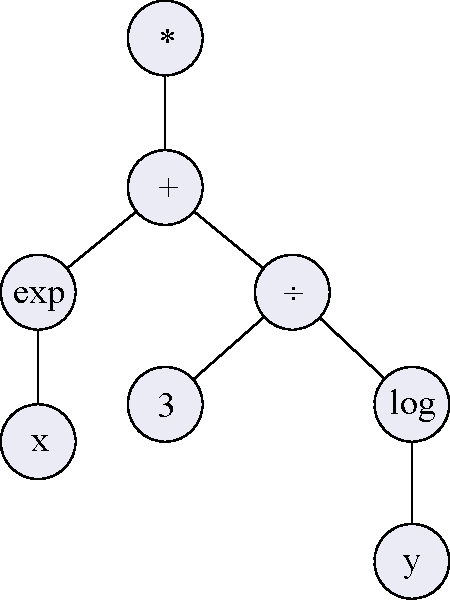
\includegraphics[height=5cm]{fig/new_tree.pdf}
	\end{figure}
	\hspace{1.7cm} $f = e^x+ \frac{3}{\log(y)}$
\end{columns}
\end{frame}

\begin{frame}{Problem statement}
	\begin{block}{Meta learning dataset}
		Let the set of pairs $\mathfrak{D} = \{D_i = (\mathbf{X}_i, \mathbf{y}_i), f_i\}_{i=1}^m$ be the data for the meta learning problem. The following conditions are satisfied:
		\begin{itemize}
			\item $\text{dom}(\mathbf{x}_i) = \text{dom}(\mathbf{x}_j)\ \forall i, j$ (all $\mathbf{X}$ share the same domain)
			\item $f_i$ is an optimal model for the base problem $D_i$ in a model space $\mathfrak{F}$:
			\[f_i = \argmin_{f \in \mathfrak{F}} \text{MSE}(\mathbf{y}_i, f_i(\mathbf{X}_i))\]
		\end{itemize}
	\end{block}
	\begin{block}{Meta learning problem}
		Given the meta learning dataset $\mathfrak{D}$, find the optimal meta model $\mathfrak{g}: D \rightarrow f$ which minimizes the error on all base problems:
		\[\mathcal{L}(\mathfrak{g}, \mathfrak{D}) = \frac{1}{m}\sum_{i=1}^m MSE(\mathbf{y}_i, \mathfrak{g}(D_i)(\mathbf{X}_i))\]
	\end{block}
\end{frame}

\begin{frame}{Solution}
	In order to solve meta learning problem we define the representations for base problem dataset $D$ and model $f$.
	\begin{block}{Model representations}
	\begin{enumerate}
		\item Symbolic expression of $f$
		\item Tree $\Gamma_f$
		\item Adjacency matrix $\mathbf{Z}_f$ of tree $\Gamma_f$
	\end{enumerate}
	We select $Z_f$ as a representation of a model.
	\end{block}
	\begin{block}{Base problem representation}
		The vector of concatenation $\mathbf{d} = [\text{vec}(\mathbf{X}), \mathbf{y}]^T$ is a representation of a dataset.
	\end{block}
\end{frame}

\begin{frame}{Solution}
	\begin{block}{Meta model decomposition}
		With selected representations of base problem and model, the meta model $\mathfrak{g}: D \rightarrow f$ is a mapping between the space of vectors $\mathbb{R}^n$ and the space of adjacency matrices of trees $\mathbb{Z}$.

		We decompose $\mathfrak{g}$ into two functions:
		\[f = \mathfrak{g}(D) = g_{\text{rec}}(g_{\text{clf}}(D)),\]
		which are recovery and classification functions.
	\end{block}
\end{frame}

\begin{frame}{Solution}
	\begin{block}{Classification}
		Classification function $g_{\text{clf}}: \mathbb{R}^n \rightarrow \mathbb{P}$ is a mapping between datasets and the space of probability matrices.
		\[g_{\text{clf}}(\mathbf{d}) = \mathbf{P}_f,\]
		where $\mathbf{P}_f$ is a matrix of probability of edges in a tree $\Gamma_f$. $g_{\text{clf}}$ is a classification algorithm (logistic regression, random forest).
	\end{block}

	\begin{block}{Matrix recovery}
		Classification function $g_{\text{rec}}: \mathbb{P} \rightarrow \mathbb{Z}$ is a mapping between the space of matrices of edge probabilities to the space of adjacency matrices of trees. We propose two methods for matrix recovery $g_{\text{rec}}$:
		\begin{itemize}
			\item Greedy algorithm
			\item Dynamic programming
		\end{itemize}
	\end{block}
\end{frame}

\begin{frame}{Greedy strategy}

\begin{algorithm}[H]
		\caption{Greedy algorithm}
		\label{alg1}
		\begin{algorithmic}
			\REQUIRE Matrix of the edge probabilities $\mathbf{P}$
			\ENSURE Recovered model $f$
			\STATE Initialize set of open vertices $S = \{*\}$
			\WHILE{$ S \neq \emptyset$ and maximum complexity is not reached}
			\STATE Extract vertex $i$ from $S$
			\IF{$i$ is a variable}
			\STATE \textbf{continue}
			\ENDIF
			\STATE Select vertex $j=\argmax_j \mathbf{P}_{ij}$ (the vertex with the highest edge probability)
			\STATE Grow tree $f$ with edge $(i, j)$
			\STATE Add $j$ to the set of open vertices $S$
			\ENDWHILE
		\end{algorithmic}
	\end{algorithm}
\end{frame}

\begin{frame}{Dynamic programming}

\begin{algorithm}[H]
	\caption{Recursive procedure $r(\mathbf{P}, f, i)$}
	\label{alg2}
	\begin{algorithmic}
		\REQUIRE Matrix of the edge probabilities $\mathbf{P}$; current tree $f$; leaf vertex~$i$ of $f$
		\ENSURE $\hat{f}, s(\hat{f})$. \enspace $\hat{f}$ is the best continuation of $f$ and has $i$ as its root.
		\IF{$i$ is a variable}
		\RETURN  $i$, $1$
		\ENDIF
		\FOR{each unused vertex and variable $j$}
		\STATE $f_j = f + (i, j)$ \enspace (grow tree $f$ with the edge $(i, j)$)
		\STATE $\hat{f_j}, s(\hat{f_j}) = r(P, f_j, j)$ \enspace (find optimal continuation for $f_j$)
		\ENDFOR
		\STATE $\hat{f} = \argmax_{f_j} s(\hat{f_j} + (i, j))$ \enspace (select optimal continuation for $f$)
		\STATE $s(\hat{f}) = \max_{f_j} s(\hat{f_j} + (i, j))$
		\RETURN $\hat{f}, s(\hat{f})$
	\end{algorithmic}
\end{algorithm}
\end{frame}

\begin{frame}{Dynamic programming}
\begin{block}{Choice of scoring function}
	\begin{itemize}
		\item $s(f) = \prod\limits_{e \in f} P_{e}$, i.e. the product of all edges probabilities, we call it tree likelihood;
		\item $s(f) = \frac{1}{n}\sum\limits_{e \in f} P_{e}$, i.e. score is the average probability of the edges in the tree.
	\end{itemize}
	The former score function penalizes deep trees heavily, while the latter allows more complex models.
\end{block}
\end{frame}

\begin{frame}{Dynamic programming}
\begin{block}{Bellman's principle of optimality.}
	An optimal policy has the property that whatever the initial state and initial decision are, the remaining decisions must constitute an optimal policy with regard to the state resulting from the first decision.
\end{block}

\begin{block}{Corollary}
\textit{Algorithm 2 satisfies Bellman's principle of optimality.}\\
% \textit{Proof.} Consider arbitrary step of the algorithm. The initial state is a given tree $f'$ and initial decisions are vertex choices that lead to the construction of such tree.
%
% Then the algorithm finds the best subtree given the initial state, thus satisfying principle of optimality. \qedsymbol
\end{block}
\end{frame}

\begin{frame}{Experiment}
The experiment was conducted on the synthetic data.
\begin{block}{Experiment scheme}
	\begin{enumerate}
		\item Generate $\approx 5000$ 1-D base problems
		\begin{itemize}
			\item $\mathbf{X}$ is uniformly distributed on $[-1, 1]$
			\item $f$ is a randomly generated non-parametric mathematical expression
			\item $\mathbf{y} = f(\mathbf{X}) + \mathcal{N}(0, 0.05)$
		\end{itemize}
		\item Split base problems into train and test set
		\item Train $g_{\text{clf}}$ on a train set
		\item Predict matrices of edge probabilities $\mathbf{P}$ for test base problems and recover models from them using $g_{\text{rec}}$
	\end{enumerate}
\end{block}
\end{frame}

\begin{frame}{Performance on base problems from test set}
	\begin{figure}[!ht]
		\centering
		\subfloat{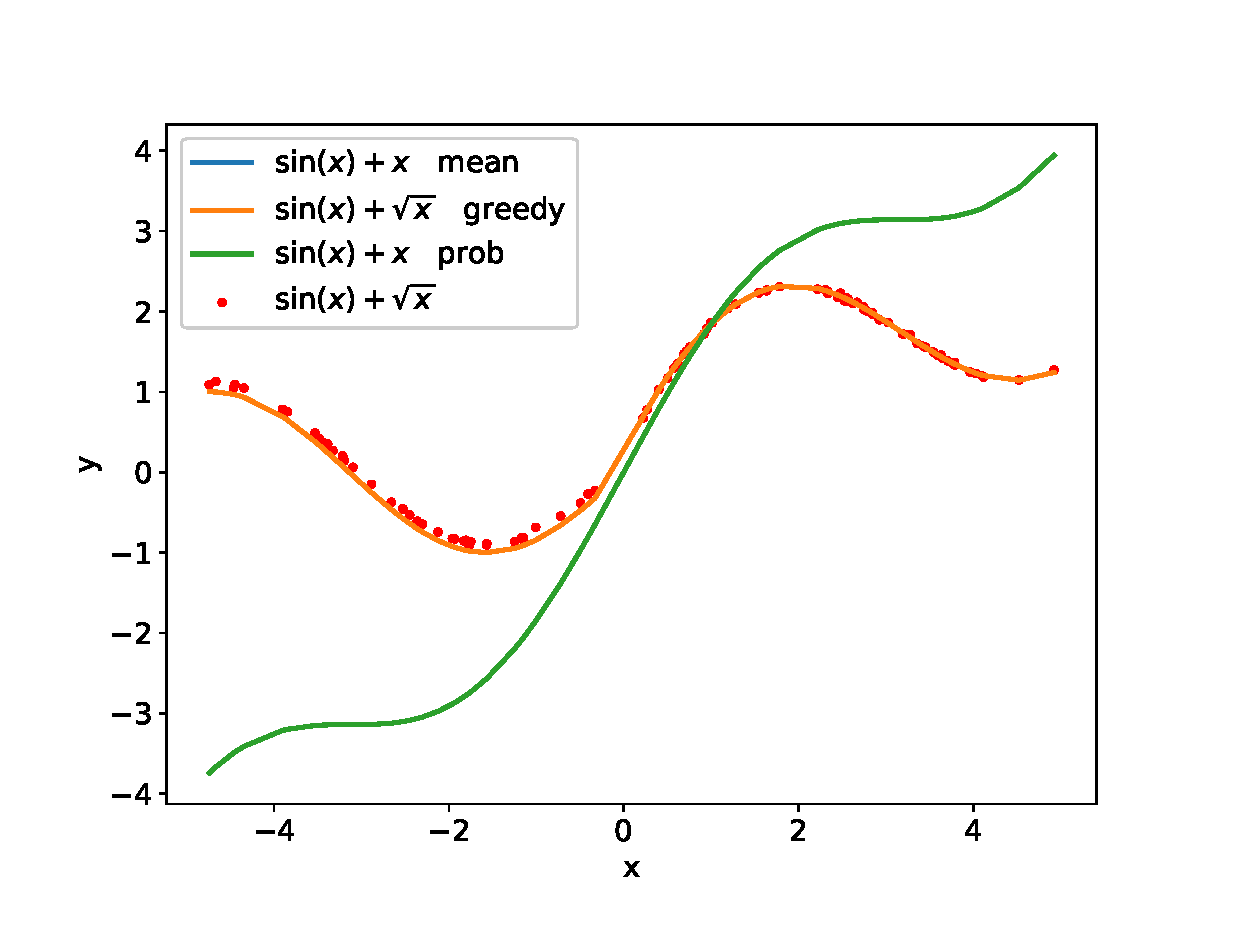
\includegraphics[width=.4\textwidth]{fig/_non_param_1.eps}}\quad
		\subfloat{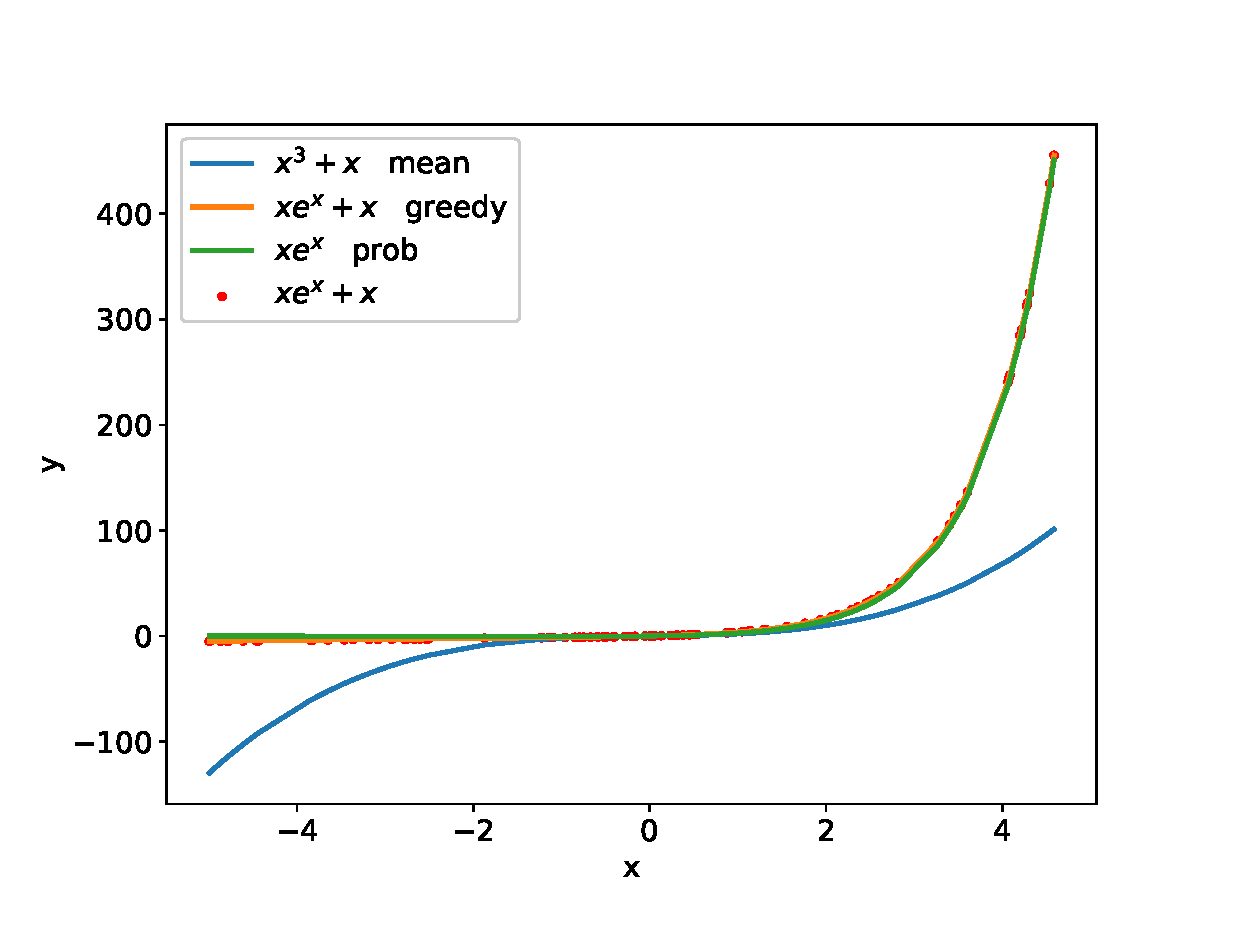
\includegraphics[width=.4\textwidth]{fig/_non_param_2.eps}}\\
		\subfloat{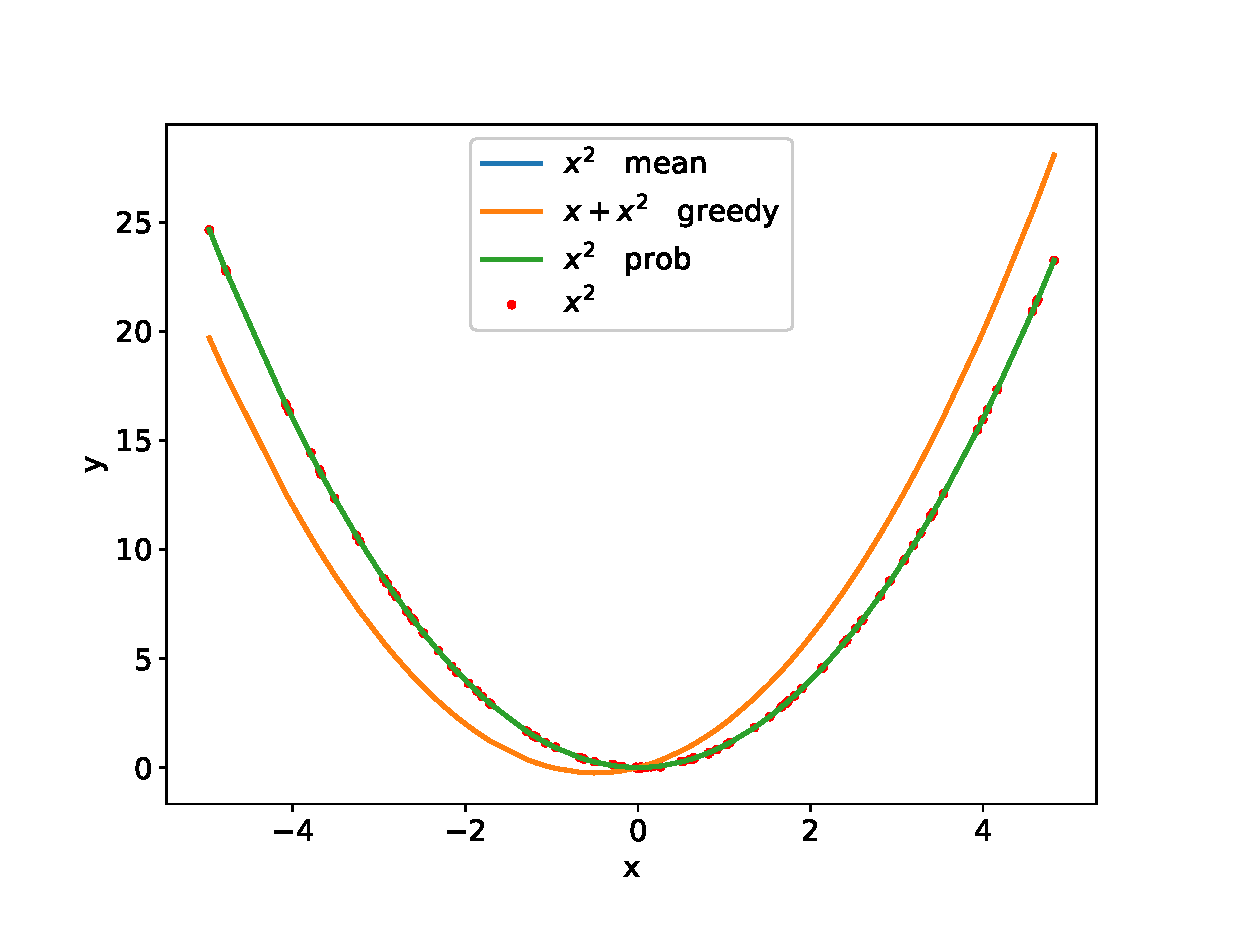
\includegraphics[width=.4\textwidth]{fig/_non_param_3.eps}}\quad
		\subfloat{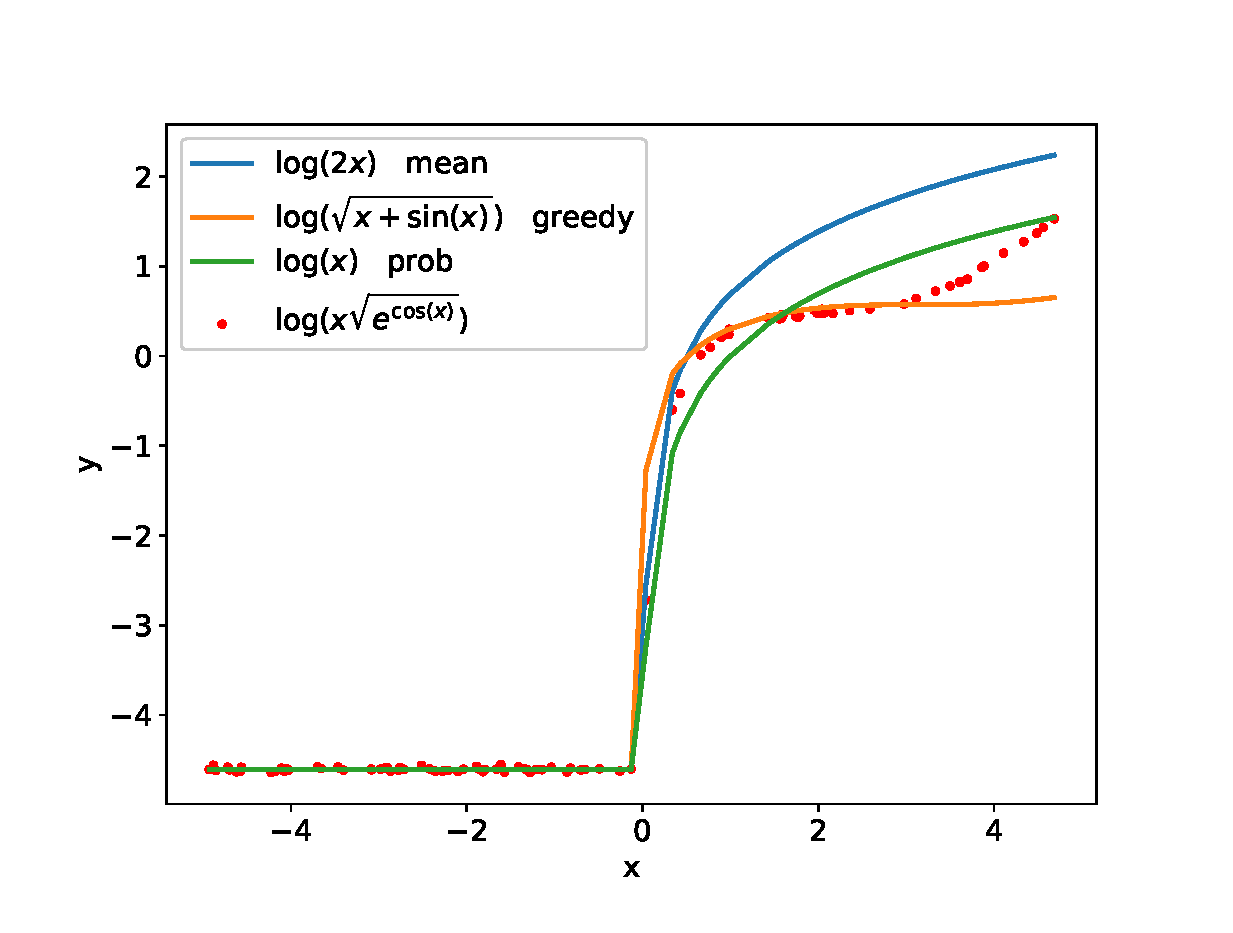
\includegraphics[width=.4\textwidth]{fig/_non_param_4.eps}}
	\end{figure}
\end{frame}

\begin{frame}{Parametric approach}
	In order to approximate real datasets we introduce parametric approach.
	Let the best non-parametric model be $f = f_1 \circ \dots \circ f_n$.

	\begin{block}{Parametrization}
		Introduce parameters for each primitive function $f_i$:
		$$f_i(\mathbf{x}, \alpha_{i1}, \alpha_{i0}) = \alpha_{i1} f_i(\mathbf{x}) + \alpha_{i0}.$$
		The function $f$ is now parametrized with parameters of its primitives:
		$$f(\mathbf{x}) \rightarrow f(\mathbf{x}, \bm{\alpha})$$
	\end{block}
	The resulting function is differentiable, vector of parameters $\bm{\alpha}$ is found using gradient descent.
\end{frame}

\begin{frame}{Method overview}
\begin{block}{Training phase}
	\begin{enumerate}
		\item Remove constants from models $f$
		\item Train $g_\text{clf}$ to predict probability matrix $\mathbf{P}$
	\end{enumerate}
\end{block}

\begin{block}{Testing phase}
	\begin{enumerate}
		\item Predict matrix $\mathbf{P}$ using $g_\text{clf}$
		\item Recover model $f$ using $g_\text{rec}$
		\item Parametrize model $f$
		\item Find optimal parameters $\bm{\alpha}$ using gradient descent
	\end{enumerate}
\end{block}
\end{frame}

\begin{frame}{Performance of parametric approach}
\begin{figure}[!ht]
	\centering
	\subfloat{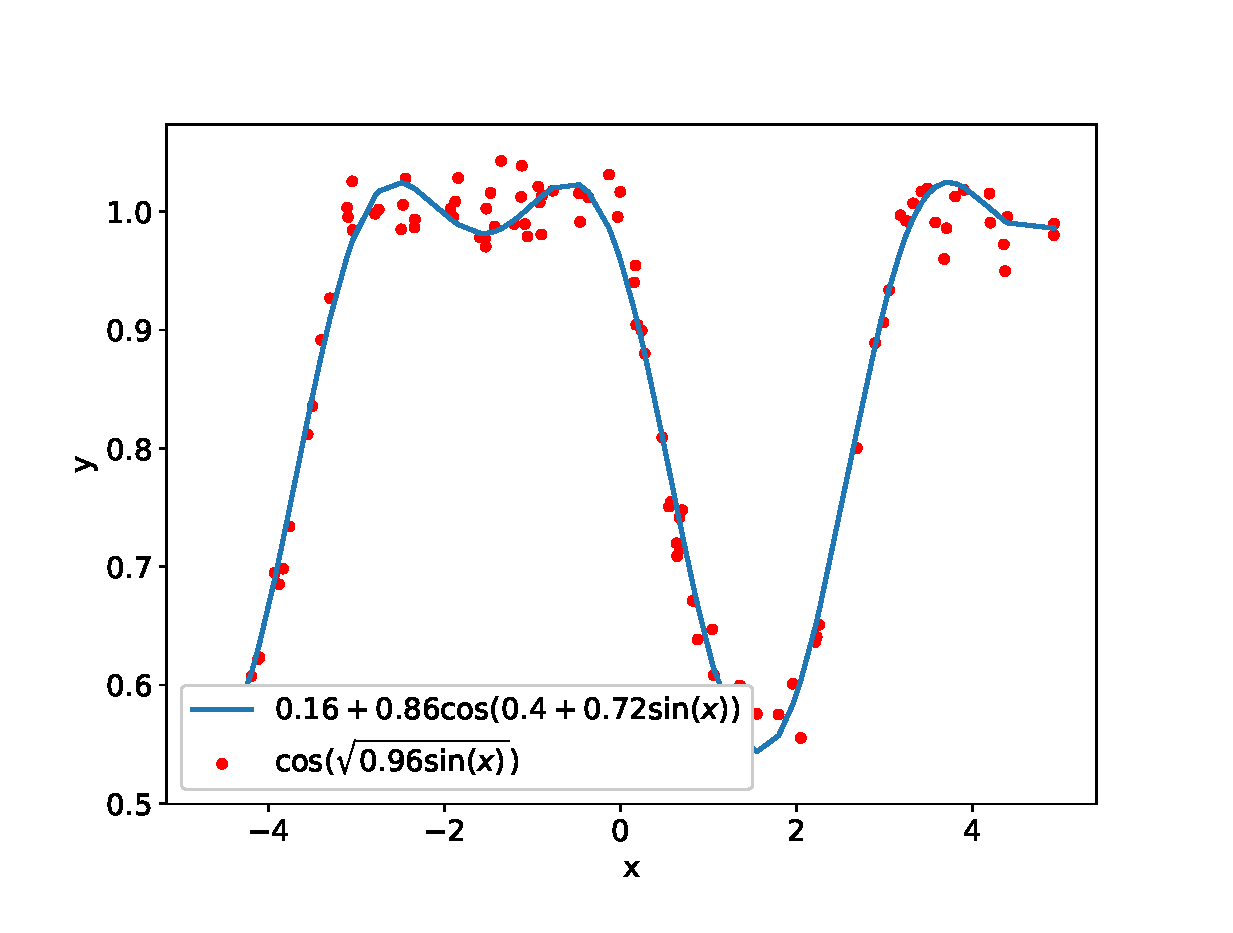
\includegraphics[width=.4\textwidth]{fig/_res_param_1.eps}}\quad
	\subfloat{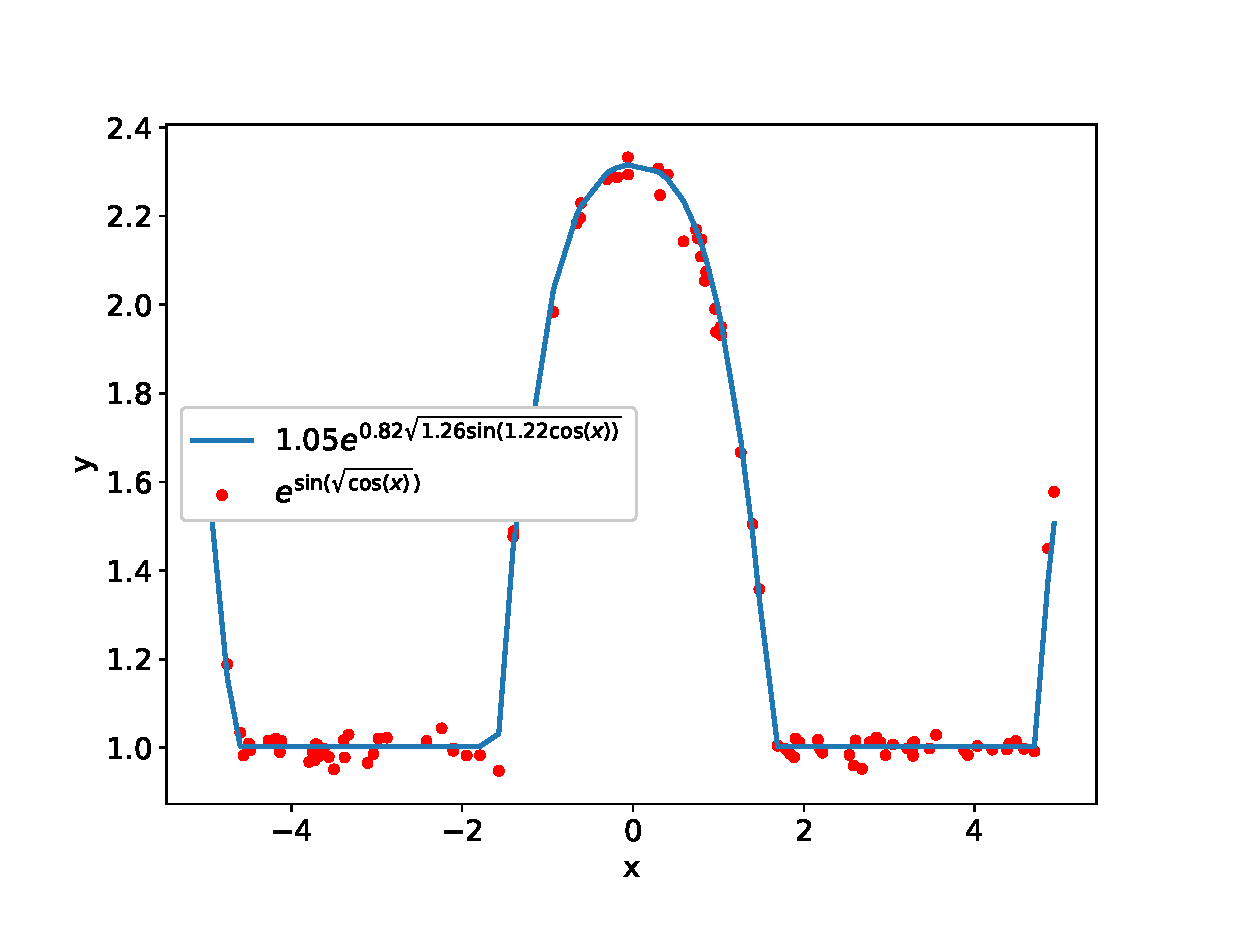
\includegraphics[width=.4\textwidth]{fig/_res_param_2.eps}}\\
	\subfloat{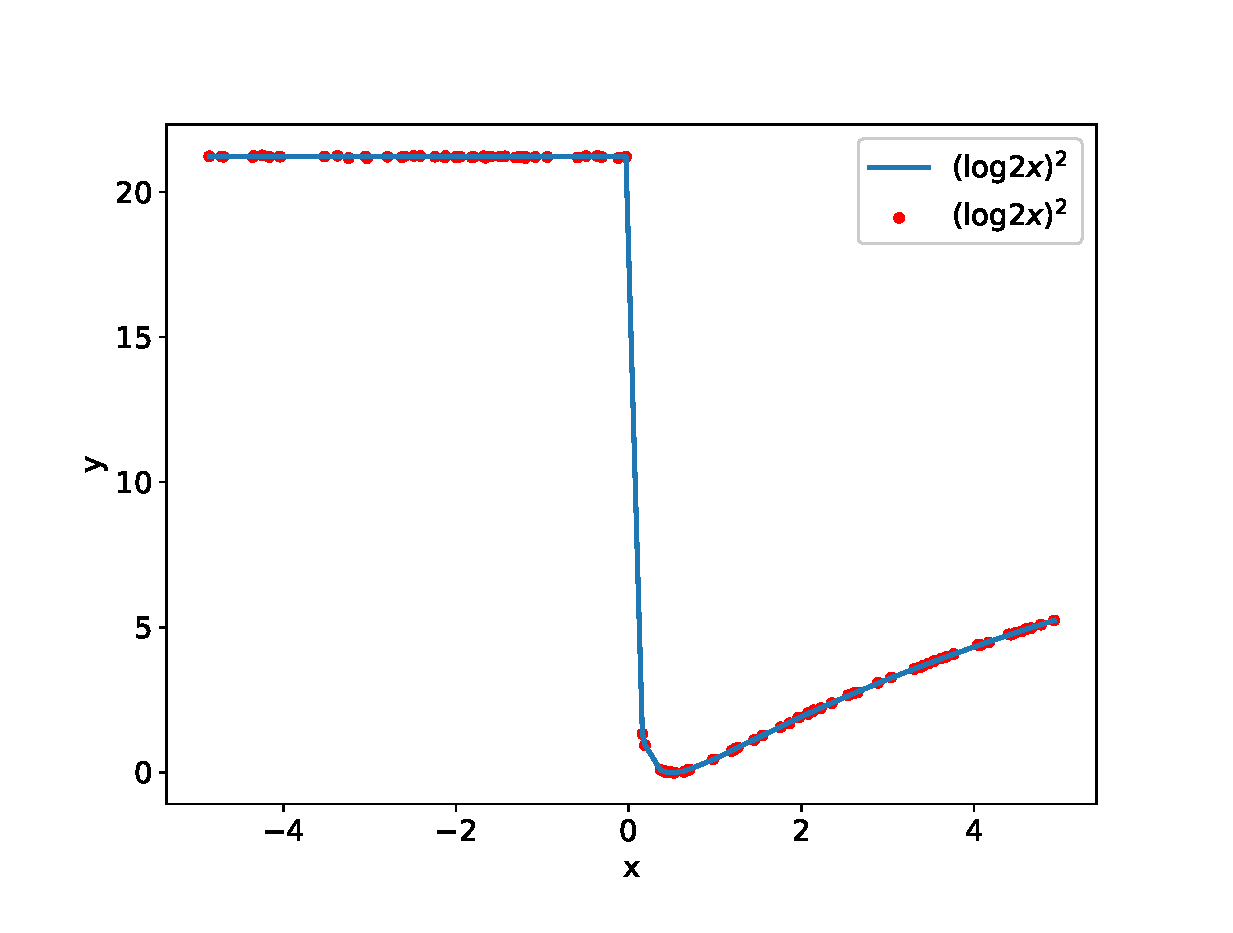
\includegraphics[width=.4\textwidth]{fig/_res_param_3.eps}}\quad
	\subfloat{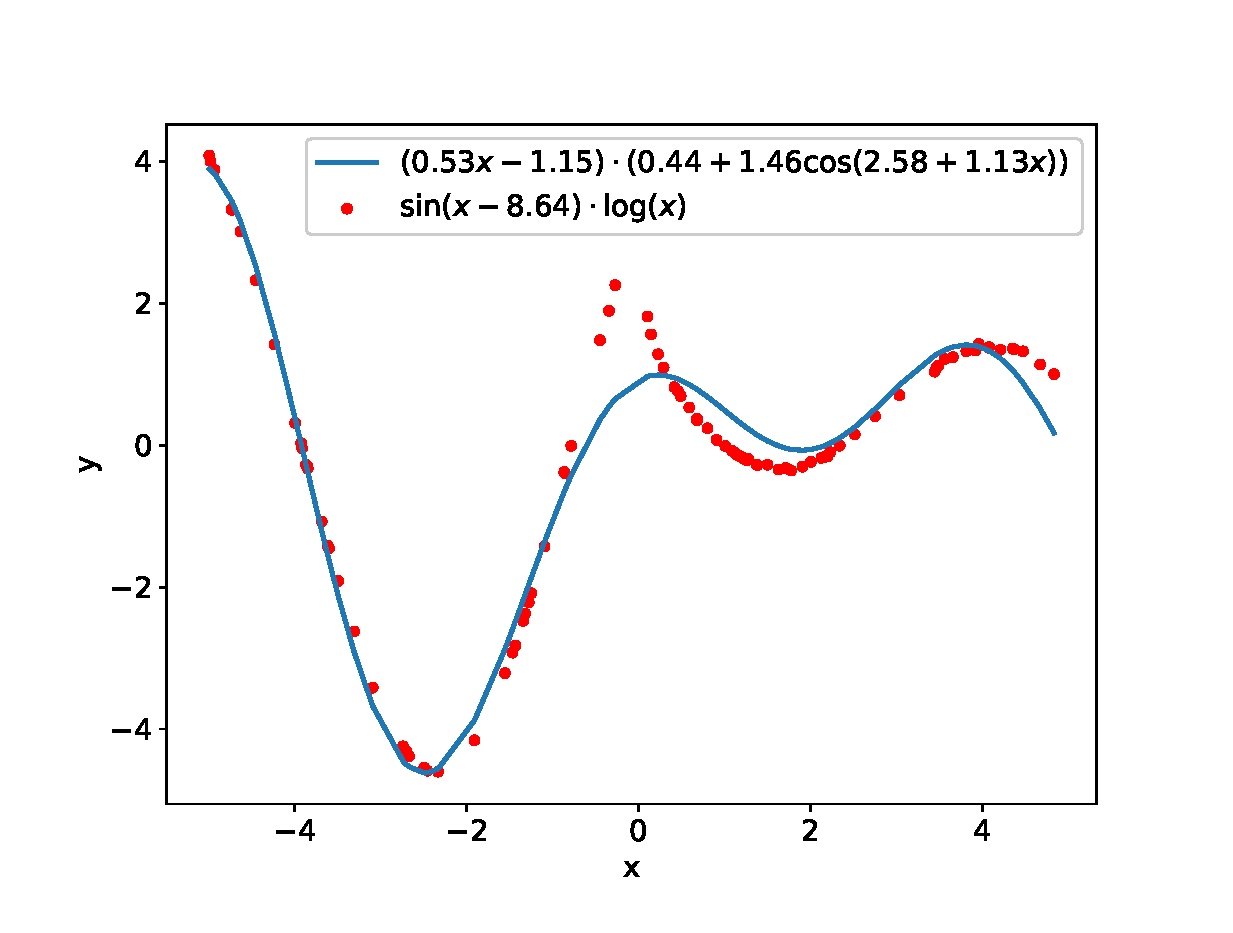
\includegraphics[width=.4\textwidth]{fig/_res_param_4.eps}}
\end{figure}
\end{frame}

\begin{frame}{Conclusions}
	\begin{itemize}
		\item Developed new framework for meta learning
		\item Conducted parametric and non-parametric experiments
		\item Method produces parametric symbolic models of good quality
	\end{itemize}
\end{frame}

\end{document}
